\section{Medium Access}
%
From the discussed model we will compare different medium access (MAC) protocols across the network and relate their performance.  The MAC protocols we are examining are CSMA, Aloha, TDMA, and FDMA.  Each MAC scheme has specific advantages over the others in different operating environments, and individually require additional mechanisms to be maintained.  The goal of our comparison is to understand how these MAC protocols can be fairly compared, and second be usefully evaluated from network and single node perspectives.  This comparison will rely upon the SG framework we have previously presented.\par
%
\subsection{Slotted Aloha}
%
Slotted Aloha is one of the simplest MAC schemes for digital communications.  It works by dividing the operation channel into time slots of a fixed duration.  When a node has data to send it will send it at the beginning of the next time slot, this is done without sensing of the channel.  Aloha networks are classically modeled as a collection of Bernoulli trials with probability $p$ of transmission.  In the SG model, $p_{sa}$ is used as a thinning factor of the PPP $\Phi_{sc}$, generating a second PPP $\Phi_{sa}$ with smaller intensity $\lambda_{sa} = p_{sa}\lambda_{sc}$.  From an interference perspective, interference observed by a given node is reduce by $p_{sa}$ on average, but the node's throughput will also be reduced by $p_{sa}$ as well, since a node cannot also be transmitting under this MAC assumption.
\par
%
From $\Phi_{sa}$ we can derive the throughput under the Slotted Aloha MAC model.  Throughput is defined as the number of successful transmissions per unit area defined in equation~\eqref{eq:throughput_slotted_aloha}, where $F_n$ is the CCDF of a standard normal.  This is a very understandable network wide metric, but it is also an average.  Throughput cannot be generalized to a single node, but is instead a spatial metric of the mean throughput averaged over all spatial configurations.  Equation~\eqref{eq:throughput_slotted_aloha} can be read as the intensity of attempted transmissions per unit area ($\lambda_{sa}$) thinned by the success probability ($1 - q(\lambda_{sa})$) of each transmission.
%
\begin{equation}\label{eq:throughput_slotted_aloha}
	\begin{split}
		T_{sa}(\lambda_{sa}) &= \lambda_{sa}(1-q(\lambda_{sa})) \\
		&=  2\lambda_{sa}(1-F_{N}\Bigg( \sqrt{ \frac{\pi/2}{ \frac{u^{-4}}{\tau} - \frac{N}{P} } } \pi \lambda_{sa} \Bigg))
	\end{split}
\end{equation}
%
Unfortunately equation~\eqref{eq:throughput_slotted_aloha} still requires a selection of the aloha transmission probability, which is contained in the input parameter $\lambda_{sa}$\footnote{$\lambda_{sa} = p_{sa}\lambda_{sc}$}.  Therefore in-order to maximum throughput for a given network intensity $\lambda_{sc}$, we must select an appropriate $p_{sa}$.  In this context, throughput is upper bounded as shown in equation~\eqref{eq:throughput_upper_bound}.
%
\begin{equation}\label{eq:throughput_upper_bound}
	\begin{split}
	T_{sa}(\lambda_{sa}) &= 2\lambda_{sa}(1-F_{N}\Bigg( \sqrt{ \frac{\pi/2}{ \frac{u^{-4}}{\tau} - \frac{N}{P} } } \pi \lambda_{sa} \Bigg)) \\
	&= \lambda_{sa} e^{-\lambda_{sa} \pi ( (\frac{\pi/2}{ \frac{u^{-4}}{\tau} - \frac{N}{P} } )^{-2/\alpha}- \epsilon^2) }
\end{split}
\end{equation}
%
The optimal value for $\lambda_{sa}$ is $1$, which is found by understanding the non-spatial reuse case (single collision domain).  In this domain throughput is simply $T_{sa}^{sd} = Np(1-p)^{N-1}$, where N is the number of accessing nodes.  The optimal value for $p$ is $1/N$, assuming if $N$ is large and the taking into account the thinning $\lambda_{sa}$ ($p=\lambda_{sa}/N$), the throughput becomes equation~\eqref{eq:single_domain}.  $\lambda=1$ clearly maximizes throughput in this sense.
%
\begin{equation}\label{eq:single_domain}
	T_{sa}^{sd}(\lambda_{sa}) = \lambda_{sa} e^{-\lambda_{sa}}
\end{equation}
\par
%
\begin{figure}[H]\label{fig:aloha_max}
	\centering
	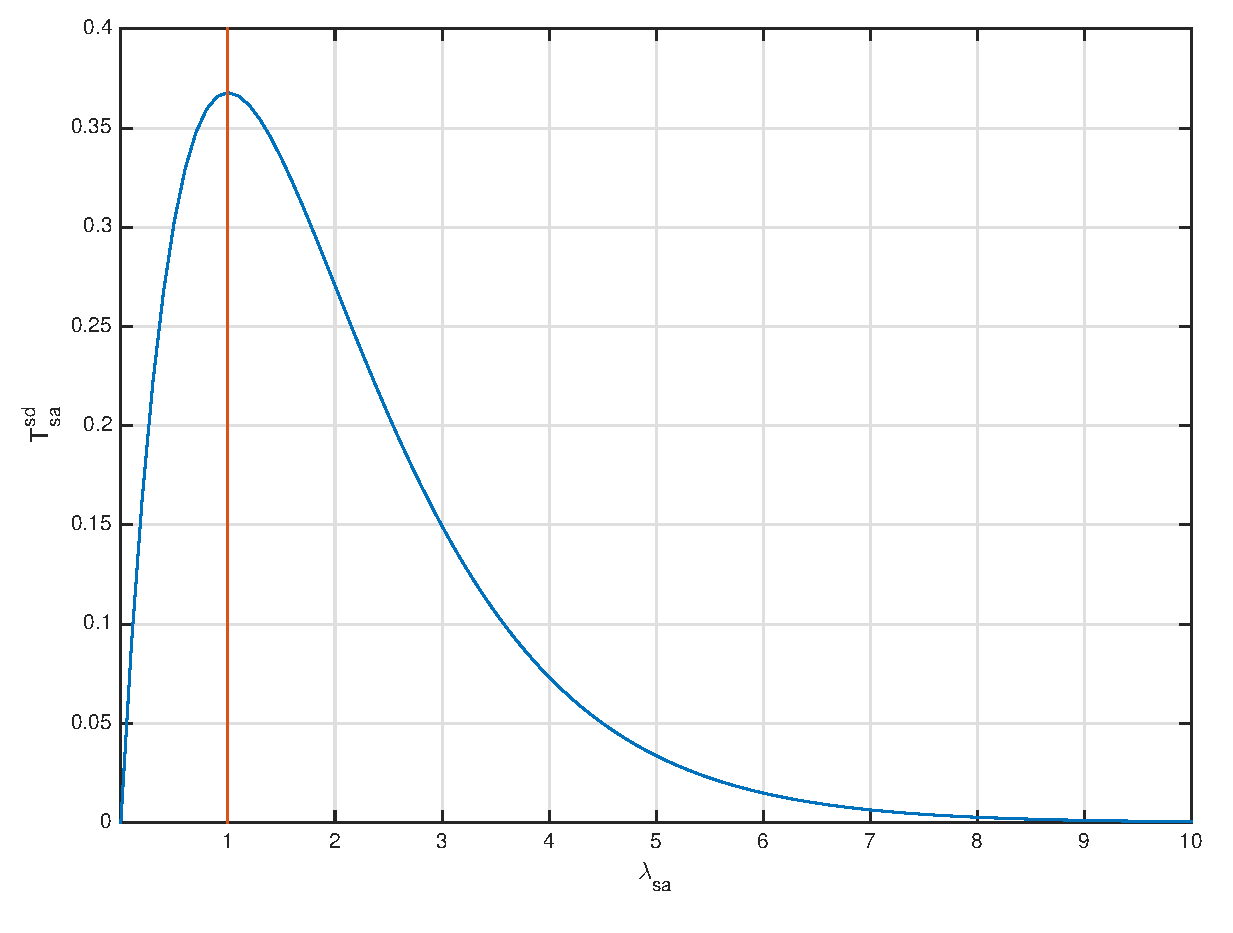
\includegraphics[width=\textwidth]{single_domain_aloha.eps}
	\caption{ss.}
\end{figure}
%
From~\eqref{eq:single_domain} the throughput becomes fixed, since $\lambda_{sa}$ is fixed.  Instead if we fix the aloha probability of transmission $p_{sa}$ at differing values and look at throughput as a function of network intensity $\lambda_{sa}$, as seen in Figure~\ref{fig:aloha_bounds}, we have a better understanding on the effects of these variables.
%
\begin{figure}[H]\label{fig:aloha_bounds}
	\centering
	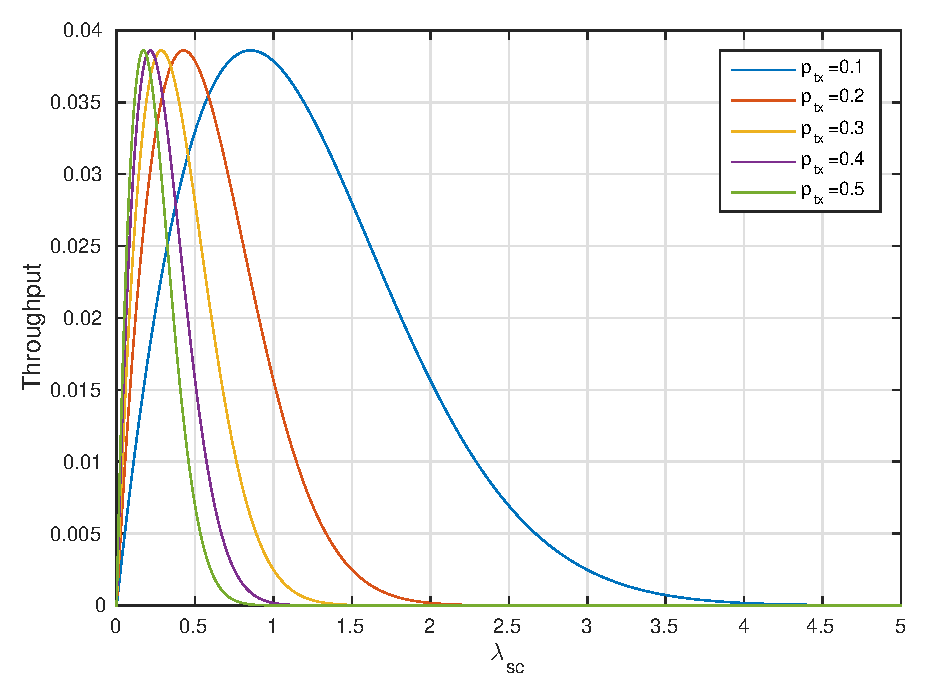
\includegraphics[width=0.75\textwidth]{aloha_throughput.eps}
	\caption{}
\end{figure}
%
\subsection{CSMA}
%
Carrier Sense Multiple Access (CSMA) is a more complicated analytical model to understand compared to Aloha since it requires point interactions.  Meaning that points have dependence on one-another in the SG framework, forcing the use of Palm distributions.  To provide some additional context into the nature of this analysis the reader must understand what is adapted in the network to reach capacity.  In slotted aloha the adjustable parameter was probability of transmission $p_{sa}$, with CSMA detection threshold instead becomes the parameter of interest.  Detection threshold takes into account the region at which nodes are allow to transmit in proximity of one another, as well as the SINR requirement at the intended receivers.  Also unlike in Slotted Aloha, in this Mat\'ern CSMA model, the probability of medium access of a typical node $p = \textbf{E}^0[e_i]$ \todo[size=\small,color=green!40]{Explain Expectation}is not given a priori and has to be determined.  $e_i$ are indicators (either $0$ or $1$) on the original PPP of transmitters $\Phi_{sc}$, marking who is allowed to transmit at a given instance.  This Mat\'ern Process defines the set of transmitters retained by CSMA
as a non-independent thinning of the $\Phi_{sc}$.
\par
%
We can compare the aloha throughput metric ($T_{sa}(\lambda_{sa})$) with a density of successful transmissions defined in equation~\eqref{eq:csma_success}. Where $r$ is the transmission distance, $\tau_0$ is the SINR threshold required at each receiver (sometimes called the detection threshold), $p_c$ is the probability of coverage, and $p_{access}$ is the probability of channel access.  \eqref{eq:csma_success} can be maximized by selecting an appropriate threshold $\tau_0$, or inversely for $r$ when fixing $\tau_0$.
%
\begin{equation}\label{eq:csma_success}
	d_{suc}(r,\tau_0) = \lambda p_c(r,\tau_0) p_{access}
\end{equation}
%

\par
%
The first step in understanding CSMA is calculating the average network-wide probability of medium access to the shared channel.  We will denote $\hat{N}$ as the average number of neighbors to a given node in the network, defined in equation~\eqref{eq:average_neighbors}.  Let us explain this thoroughly so we are not confused by the use of Palm Probabilities here.  First of all, $\textbf{E}^0$, means that the expectation is in respect to the Palm distribution $P^0$, or average perspective of points. Therefore, from the perspective of a typical node (centered at $\textbf{0}$), is we sum over all marked points in $\hat{\Phi}$ ($(X_j,m_i,F^0_j) \in \Phi$) which are marked again as follows:
%by $1$ if they meet the threshold requirement $ \Big(\frac{F_j^0}{l(|x_i-x_j|)} \geq T \Big) $ and $0$ if not.
\begin{equation}
\mathbb{1} = \begin{cases}
      1 & \frac{F_j^0}{l(|x_i-x_j|)} \geq T \\
			0 & otherwise
   \end{cases}
\end{equation}
%
Therefore the resulting $\hat{N}$ will be the average probability of having a neighboring node that is within sensing range set by $T$.  Please see Appendix~\ref{app:palm} for further details about Palm distributions.
%
\begin{equation}\label{eq:average_neighbors}
	\hat{N} = \textbf{E}^0\Bigg[ \sum_{(X_j,m_i,F^0_j) \in \hat{\Phi}} \mathbb{1}\Big(\frac{F_j^0}{l(|x_i-x_j|)} \geq T\Big) \Bigg]
\end{equation}
%
Now by applying Slivnyak’s theorem and Campbell’s (see Appendix~\ref{app:campbell}) formula we can extend~\eqref{eq:average_neighbors}.  Since $\Phi$ is stationary, Campbell’s formula simply applies~\eqref{eq:campbell_stationary} on line two, and a coordinate change on line three\todo[size=\small,color=green!40]{Review is Srikanth}.
%
\begin{equation}\label{eq:average_neighbors}
	\begin{split}
	\hat{N} &= \textbf{E}^0\Bigg[ \sum_{(X_j,m_i,F^0_j) \in \hat{\Phi}} \mathbb{1}\Big(\frac{F_j^0}{l(|x_i-x_j|)} \geq T\Big) \Bigg] \\
	&= \lambda \int_{\mathbb{R}^2} P\{ F \geq T l(|x|) \} dx \\
	&= 2 \pi \lambda \int_{0}^{\infty} (1 - G(T l(r) ) )r dr
\end{split}
\end{equation}
%
Where $G$ is the CDF of $F$.  From~\eqref{eq:average_neighbors} we can determine the probability of medium access of a typical node, shown in equation~\eqref{eq:medium_access} as the average mark of a typical point $x_0$.
%
\begin{equation}\label{eq:medium_access}
	p_{access} = \textbf{E}^0[e_0] = \frac{(1-e^{-\hat{N}})}{\hat{N}}
\end{equation}
%
This equation is a natural extension from the expectation of the void probability. Void probability, in the case of a PPP $\Phi$ with no markings, can be seen in equation~\eqref{eq:void_probability}.  Void probability is simply the probability that no points exist within radius $r$ of the the point of interest, assuming the number of points is poisson\footnote{Poisson PMF $P(k)=\frac{\lambda^k}{k!}e^{-\lambda}$}  in this case and $k=0$ (aka no points).
%
\begin{equation}\label{eq:void_probability}
	P(\Phi(b(\textbf{0},r))=0) = \int_0^r e^{-\lambda \pi r^2} =
\end{equation}
%
To find the average number of points, we simply take the expectation of~\eqref{eq:void_probability}.
%
\begin{equation}\label{eq:mean_void_probability}
	\textbf{E}\big[P(\Phi(b(\textbf{0},r))=0)\big] = \frac{}{\lambda \pi r}
\end{equation}
\par
%
The probability of coverage $p_c(r,\tau_0)$ is the final piece to our throughput calculation $d_{suc}(r,\tau_0$.  Assuming the receiver of interest at the origin $\textbf{0}$, coverage probability is written as the following:
%
\begin{equation}
	\begin{split}
	p_c(r,T) &= P^0\Bigg(\frac{F}{l(r)} \geq WT + \sum_{x_i \in \hat{\Phi} \setminus 0} \frac{F_i T} {l(|x_i-z|)} |\;0 \in \hat{\Phi} \Bigg) \\
	&= P^0\Bigg( F \geq l(r) T \Bigg( W + \sum_{x_i \in \hat{\Phi} \setminus 0} \frac{F_i} {l(|x_i-z|)} \Bigg) |\;0 \in \hat{\Phi} \Bigg) \\
	&= \frac{F}{l(r) T} \geq \Bigg( W + \sum_{x_i \in \hat{\Phi} \setminus 0} \frac{F_i} {l(|x_i-z|)} \Bigg) |\;0 \in \hat{\Phi} \Bigg)
	\end{split}
\end{equation}
%
\section{Modifications}
%
Vary number of resources used by SC across different intensities.\par
%
Have a stochastic resource usages, defined by a traffic model.\par
%
